\documentclass[class=../report, crop=false]{standalone}
\usepackage{graphicx}

\begin{document}

\section{Conceptual Solutions}

We combined the generated concept fragments using a morphological chart* to form whole concepts.
Each team member selected a set of concept fragments from the morphological chart and drew their interpretation of the whole concept; this process was done twice to ensure a variety of ideas.
We decided that the concepts generated were adequately creative for our purposes.
Time spent generating a greater variety of ideas would be better used for prototyping. Some of our most creative and promising solutions are presented below\footnotemark.

\footnotetext{The entire list of concepts generated can be found in Appendix B: Concepts Generated.}

\subsection{Creative Concepts}

One of the most creative ideas we generated is The Very Hungry Caterpillar (TVHC, Figure \ref{fig:tvhc}).
TVHC has multiple carts following behind it to allow for better turning capability; furthermore, it has a potentiometer* in front to detect turns and communicate them to the Arduino (a microcontroller)*.
This segmented design primarily addresses our train’s need to corner effectively while the need to generate torque is reflected in the design’s more traditional gear transmission.

\begin{figure}[H]
	\centering
	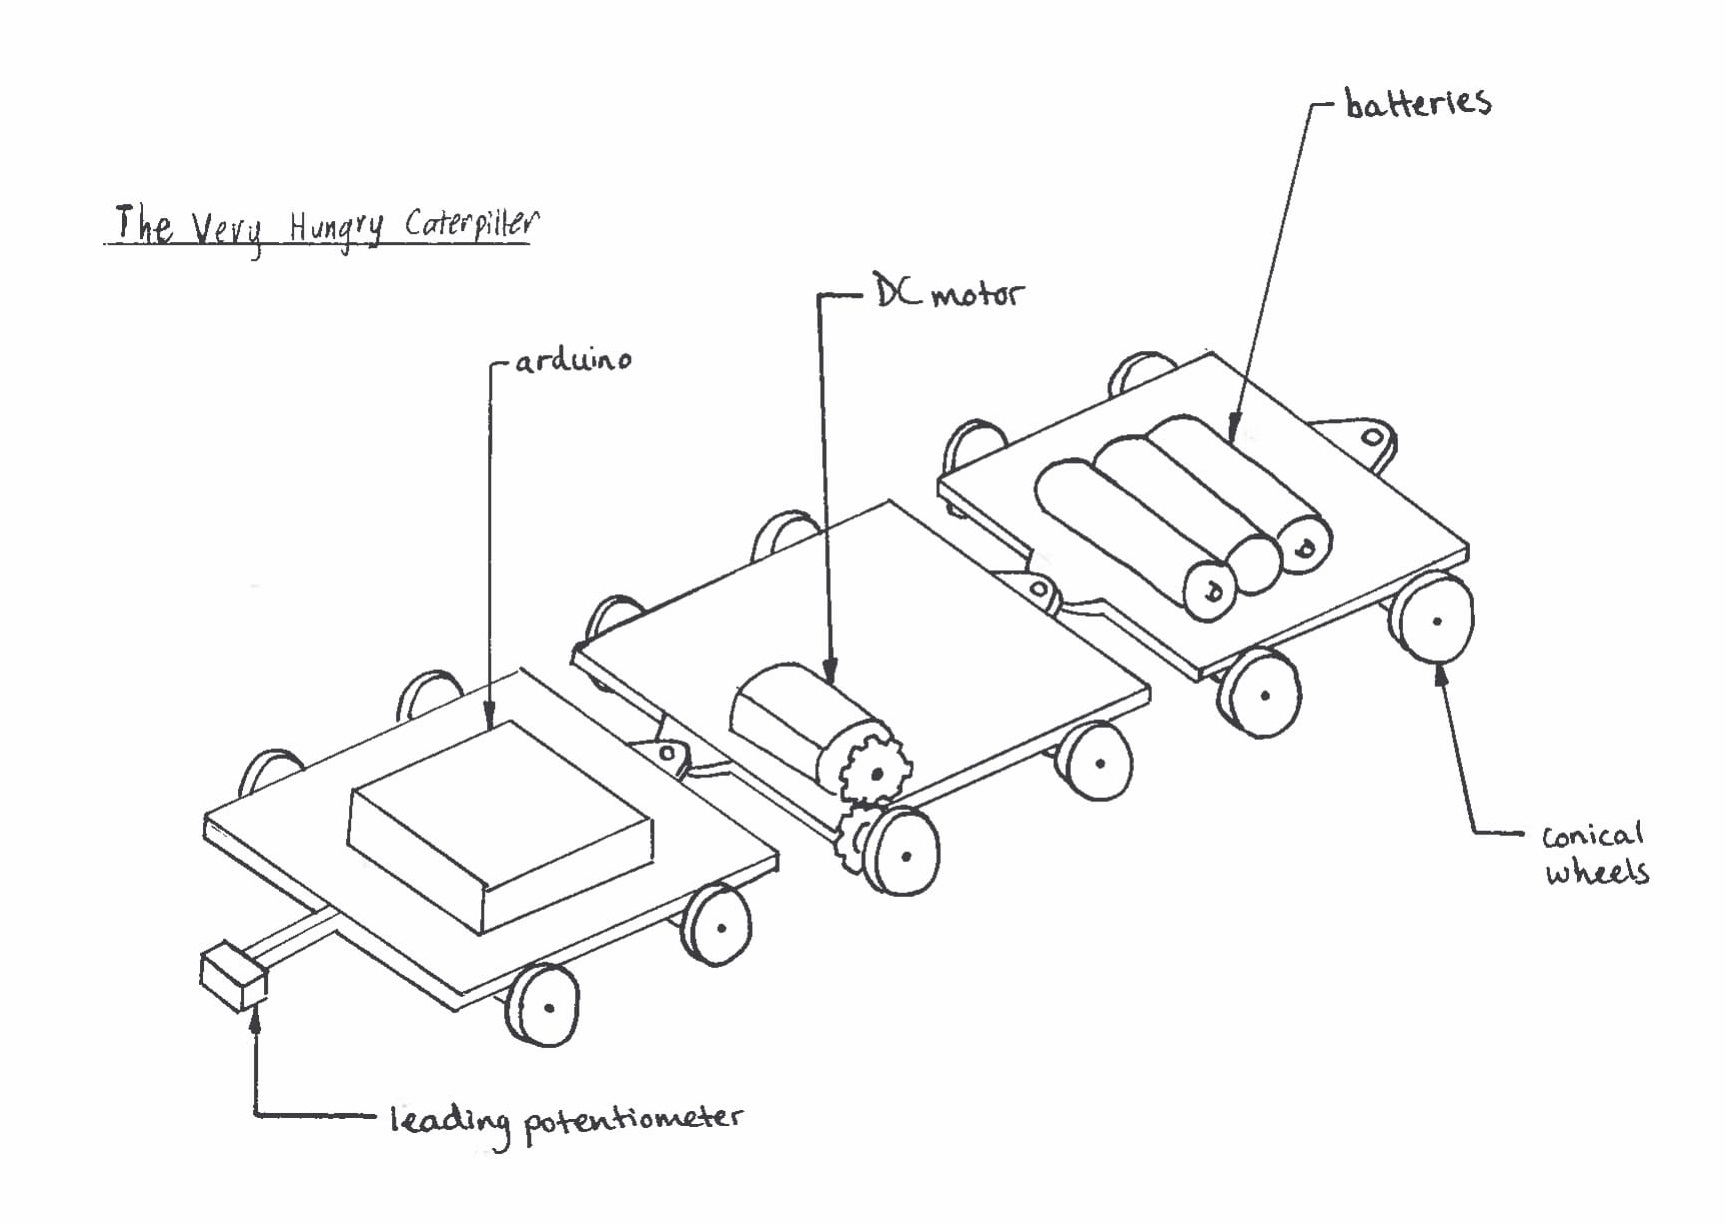
\includegraphics[width=0.8\textwidth]{../res/img/tvhc}
	\caption{TVHC (The Very Hungry Caterpillar)}
	\label{fig:tvhc}
\end{figure}

\clearpage

We created Tanky Train (Figure \ref{fig:tankytrain}) as another alternative design.
Tanky Train uses treads to drive both sets of wheels and increase friction.
The design uses direct drive to transmit torque to the treads.
This addresses our design objective of generating a high torque to climb the hills on the tracks.
It also uses a potentiometer to detect turns and a drum brake to decelerate. 

\begin{figure}[H]
	\centering
	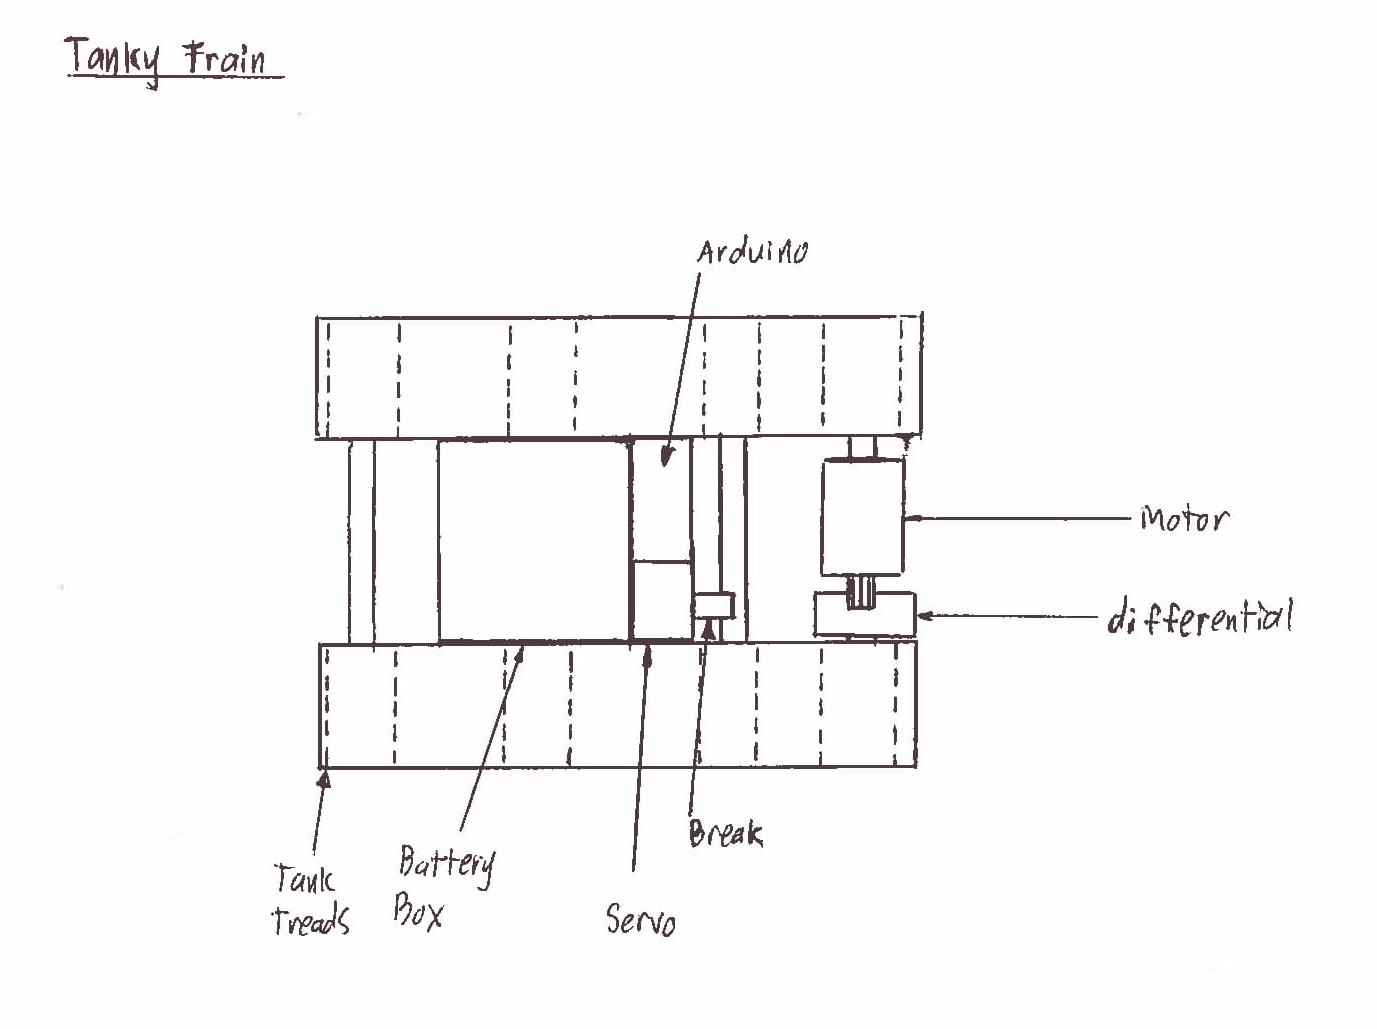
\includegraphics[width=0.8\textwidth]{../res/img/tankytrain}
	\caption{Tanky Train}
	\label{fig:tankytrain}
\end{figure}

\clearpage

\subsection{Promising Concepts}

Our most promising concept is Get Hitched (Figure \ref{fig:gethitched}).
This design drives each axle with a separate motor to increase torque.
Get Hitched is also designed to be low to the ground, increasing its cornering ability; this is further increased by the design’s use of conical wheels.
A light sensor is used for detecting its position along the track.
This design addresses both of the attributes needed to complete the rounds and achieve our design objectives.

\begin{figure}[H]
	\centering
	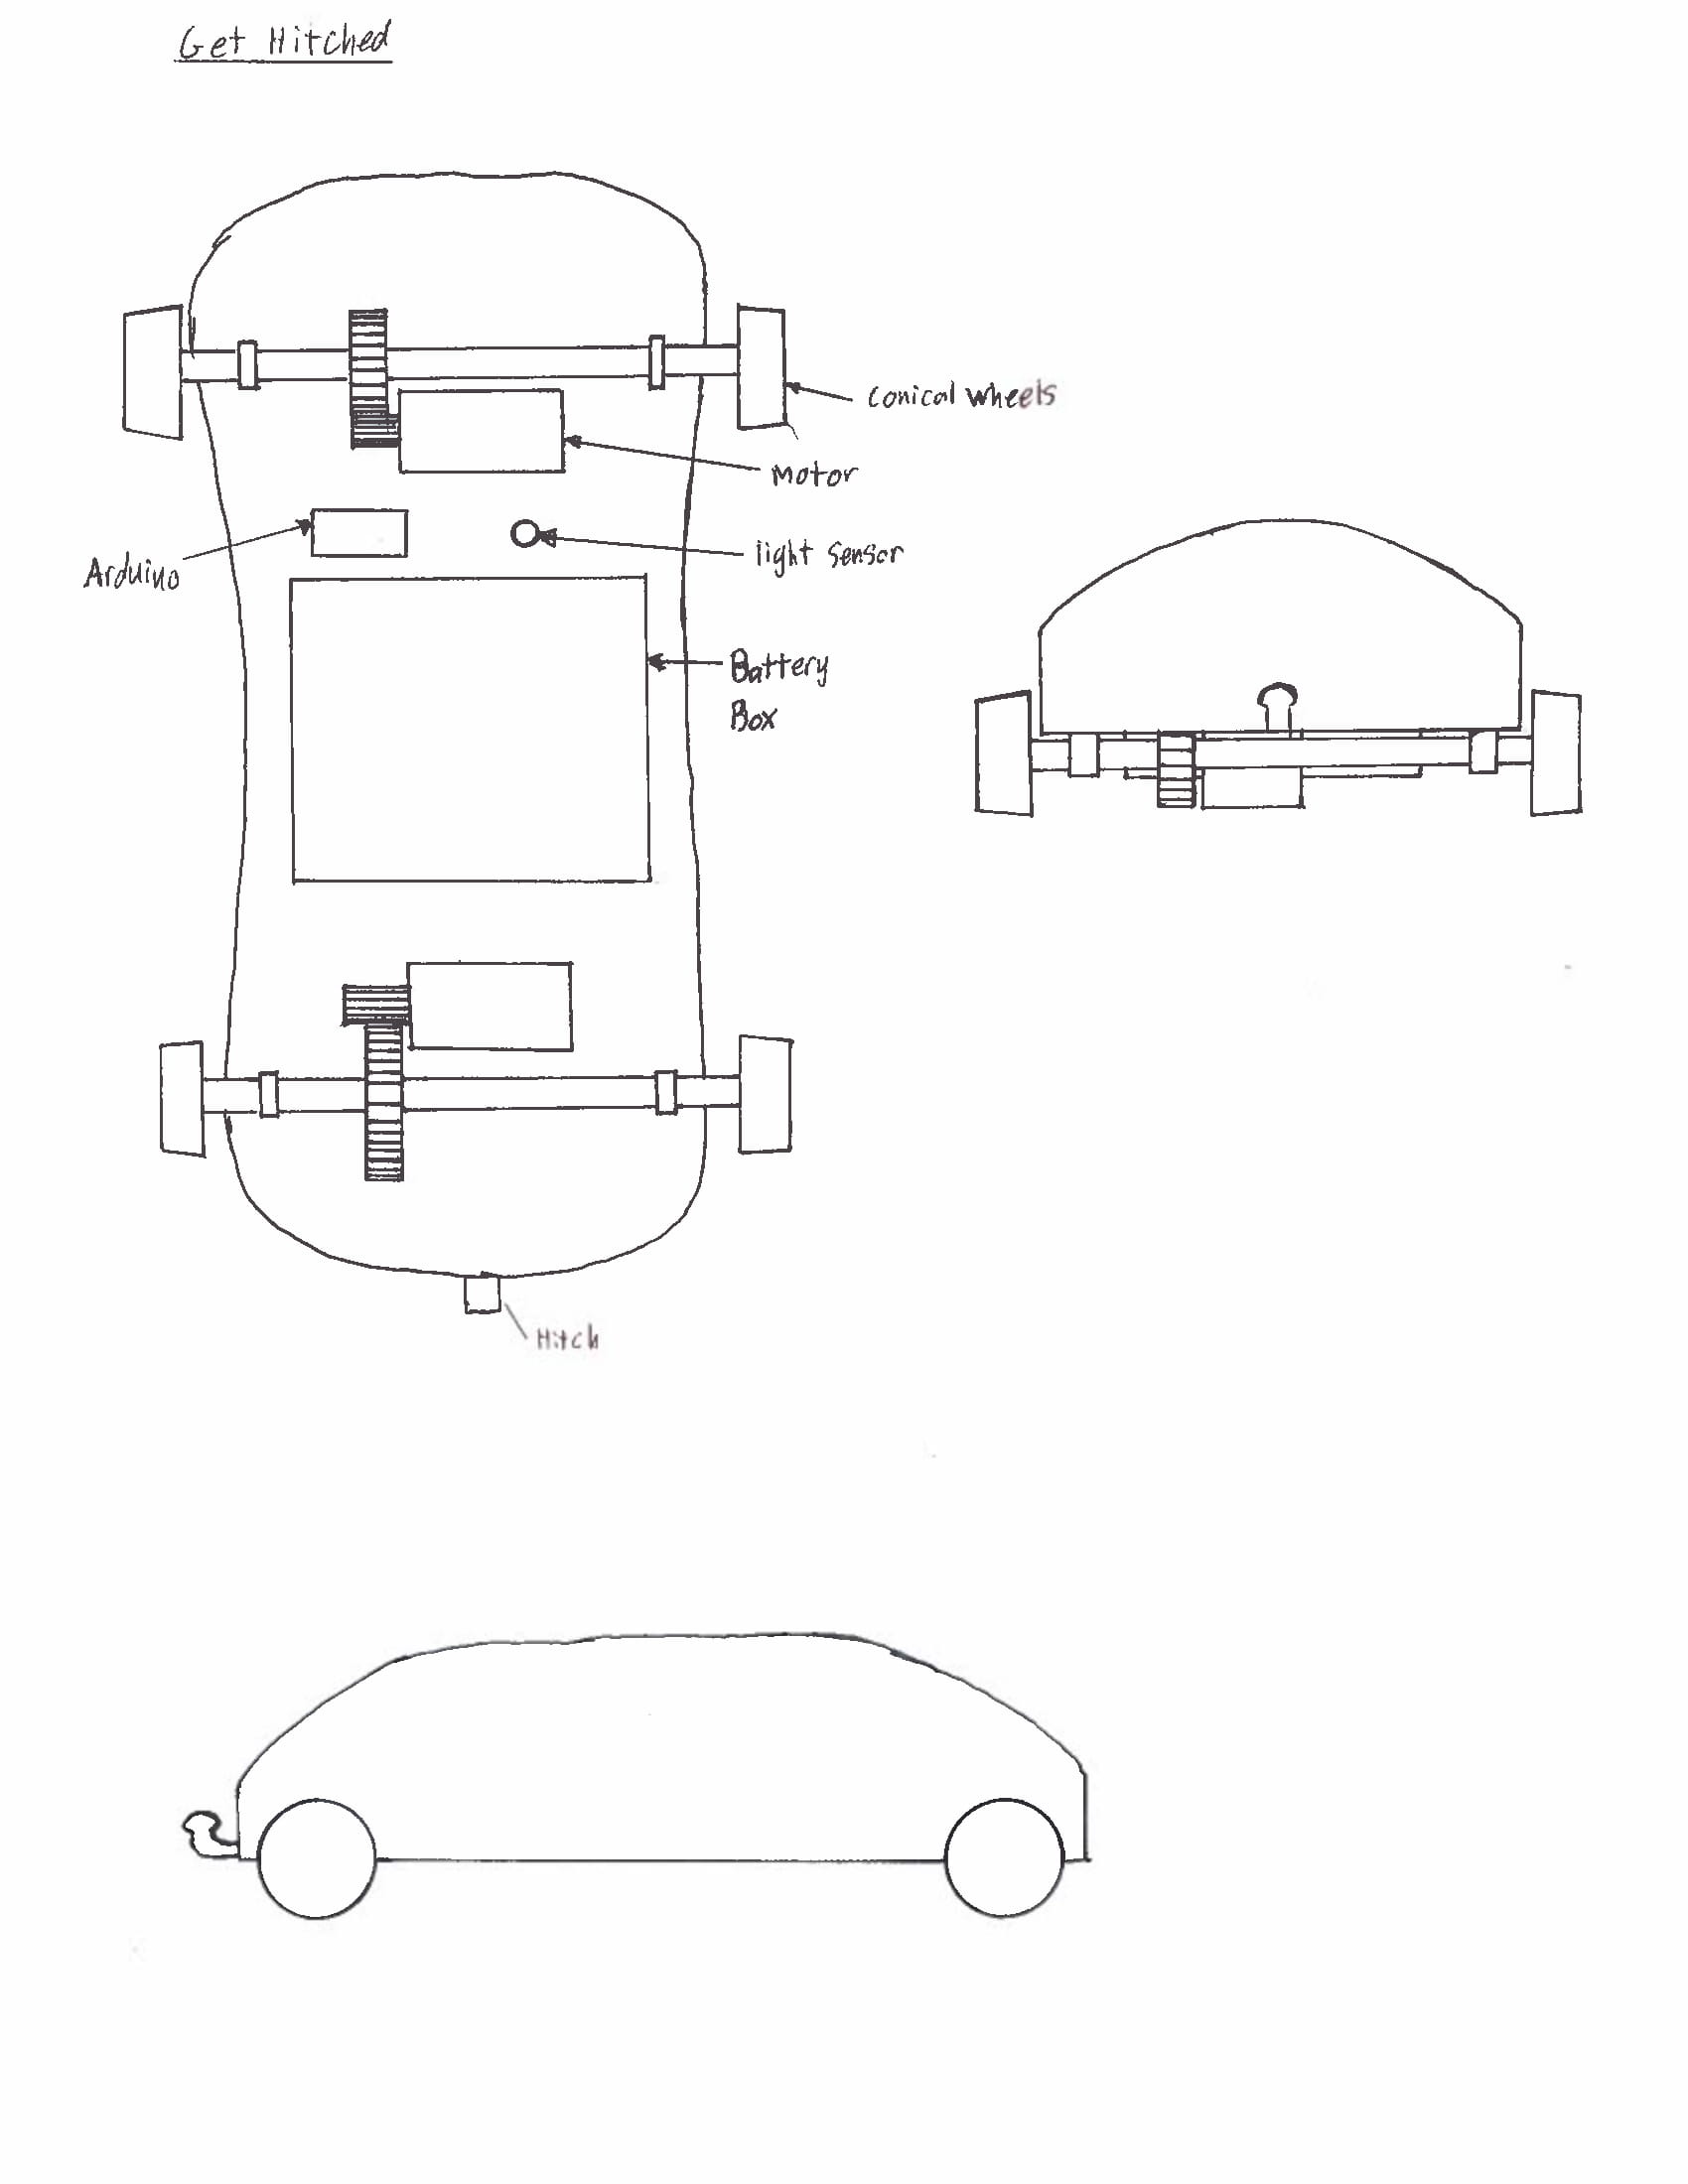
\includegraphics[width=0.8\textwidth]{../res/img/gethitched}
	\caption{Get Hitched}
	\label{fig:gethitched}
\end{figure}

\clearpage

The concept Puff (Figure \ref{fig:puff}) uses a variable gearbox to transfer the energy from the motor to the wheels.
This addresses our primary design objective of increasing torque output, while also providing the ability to increase acceleration.
It uses a potentiometer to detect turns and conical wheels to increase stability during turns.
The design is promising because it has the ability to be easily modified for different rounds.

\begin{figure}[H]
	\centering
	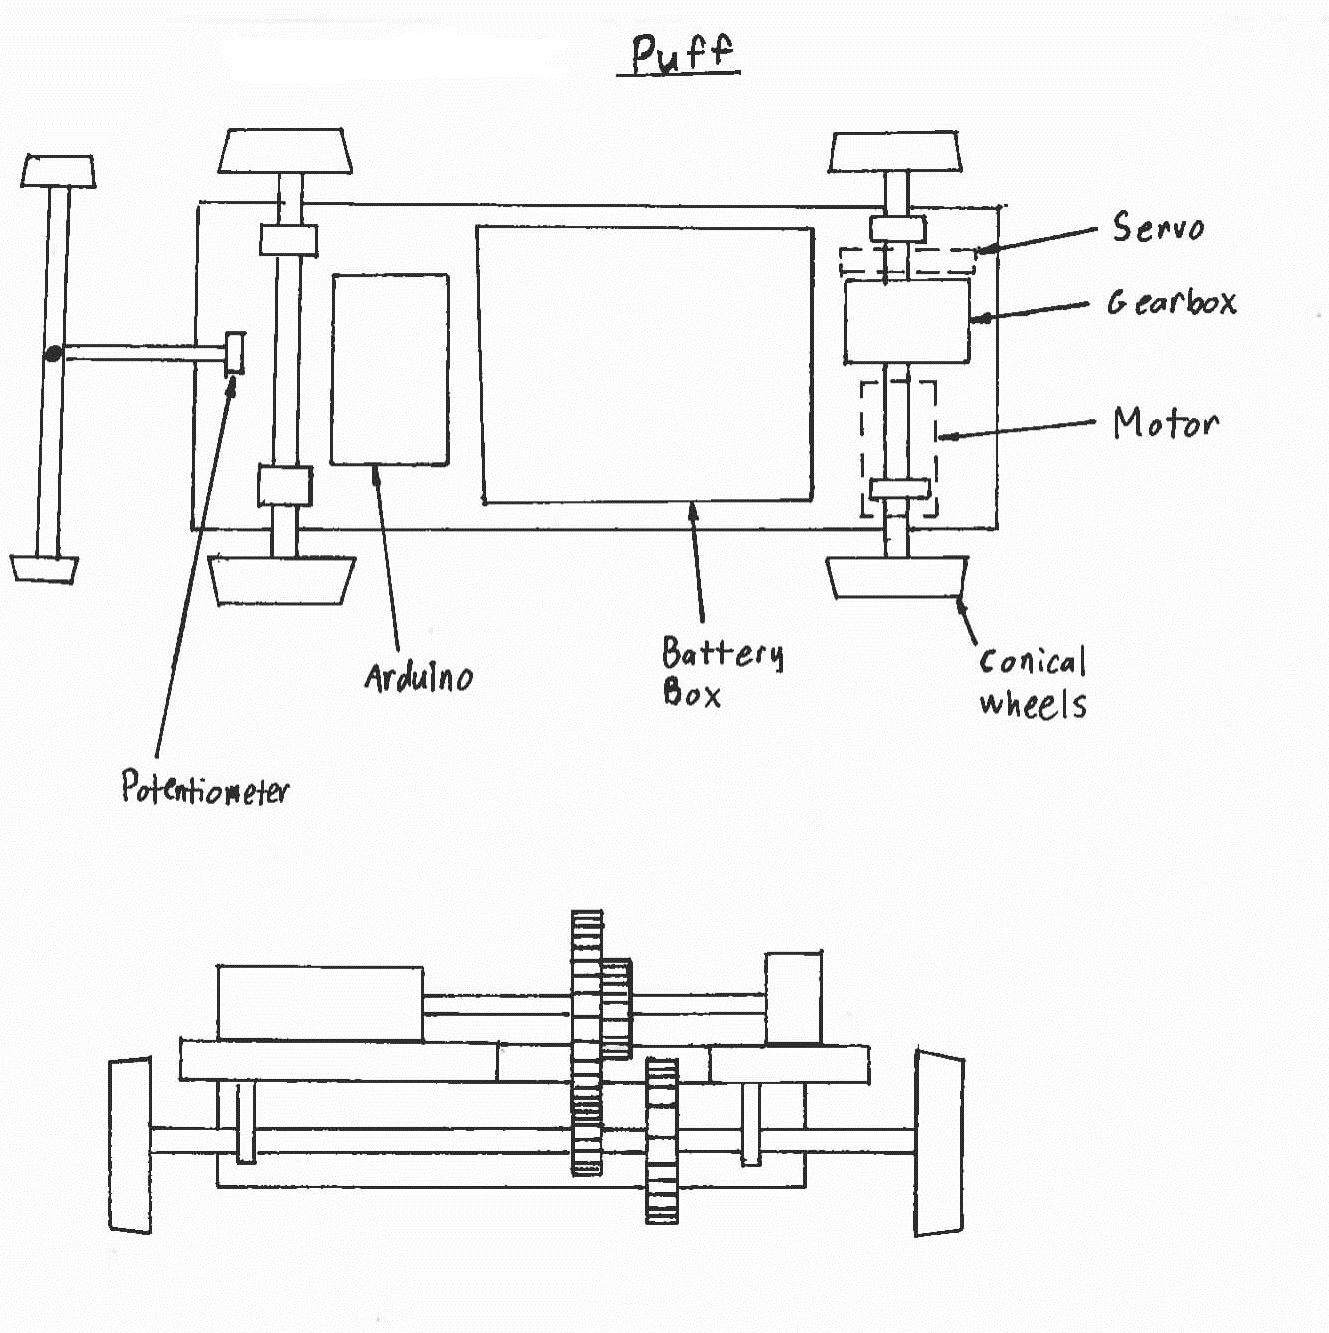
\includegraphics[width=0.8\textwidth]{../res/img/puff}
	\caption{Puff}
	\label{fig:puff}
\end{figure}

\clearpage

We also generated many promising designs such as Simplicity (Figure \ref{fig:simplicity}) that use belt drives.
It does not include a turn detection device and uses simple wheels with o-rings.
Despite poorly addressing our cornering objective, the design was simple and we were almost certain it would be built by competition.
It could also be easily modified to include complex parts once a basic prototype was created.

\begin{figure}[H]
	\centering
	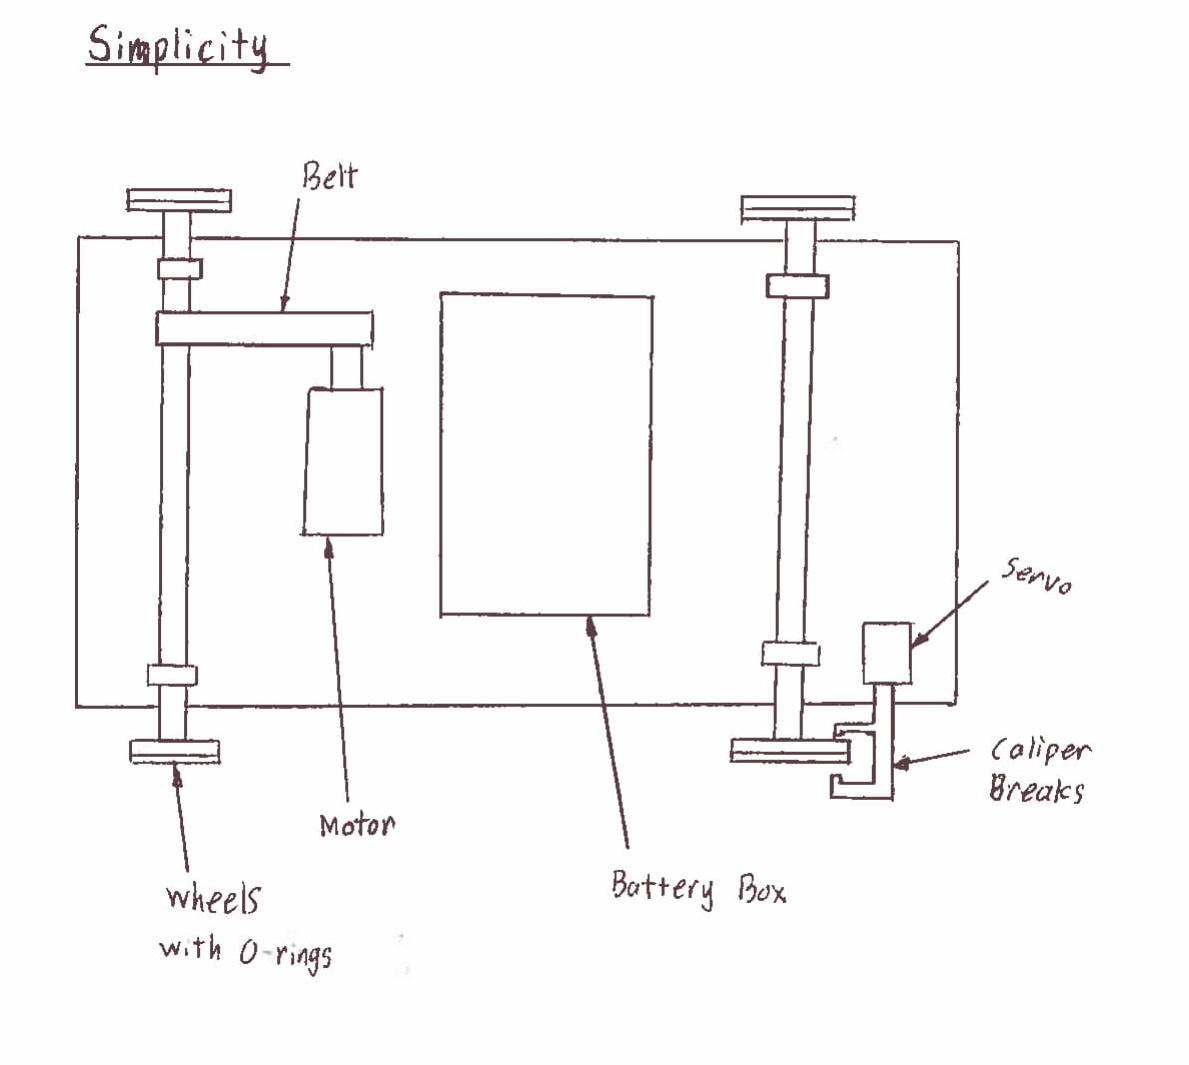
\includegraphics[width=0.8\textwidth]{../res/img/simplicity}
	\caption{Simplicity}
	\label{fig:simplicity}
\end{figure}

\end{document}
